\subsection{Performance Evaluation}
\label{sec:evaluation}
%We have compared the processing time of each user login in UPPRESSO, with the original OIDC implementation (MITREid Connect) and SPRESSO which only hides the user's accessed RPs from IdP.
\noindent\textbf{Environment.} The evaluation was performed on 3 machines,
one (3.4GHz CPU, 8GB RAM, 500GB SSD, Windows 10) as IdP,
one (3.1GHz CPU, 8GB RAM, 128GB SSD, Windows 10) as an RP,
and the last one (2.9GHz CPU, 8GB RAM, 128GB SSD, Windows 10) as a user.
The user agent is Chrome v75.0.3770.100.
And the machines are connected by an isolated 1Gbps network.

%RP(不包括特定方案的SDK)大约需要230行JAVA代码
%OIDC(MITREid)的SDK需要大约20行的JAVA代码,需要额外添加一个HTML文件(包含大约20行JavaScript代码)
%UPPRESSO的SDK需要大约1100行代码,不需要添加额外的HTML文件
%OIDC和UPPRESSO的SDK只需要RP提供两个网络接口(网址),然后在对应的网络接口中引用对应的API(每个接口对应一个API,分别命名为tokenRequestGenerate和userAccountAchieve),其他的处理流程均由SDK完成
%SPRESSO由于结构与OIDC完全不同,所以使用了SPRESSO提供的RP的开源代码
%For better evaluation, we build one RP for both UPPRESSO and MITREid Connect which is also implemented  based on Spring Boot framework, as well as the identity proof transmission from user to RP in MITREid Connect is implemented by JavaScript running in RP's web page. The IdP in MITREid Connect is achieved from github~\cite{MITREid}. However, the SPRESSO system is downloaded from~\cite{spressome} containing IdP, RP and FWD.

%A DELL OptiPlex 9020 PC (Intel Core i7-4770 CPU, 3.4GHz, 500GB SSD and 8GB RAM) with Window 10 prox64 works as the IdP. A ThinkCentre M9350z-D109 PC (Intel Core i7-4770s CPU, 3.1GHz, 128GB SSD and 8GB RAM) with  Window 10 prox64 servers as RP. The user adopts Chrome v75.0.3770.100 as the user agent on the Acer VN7-591G-51SS Laptop (Intel Core i5-4210H CPU, 2.9GHz, 128GB SSD and 8GB RAM) with  Windows 10 prox64. For SPRESSO, the extra trusted entity FWD is deployed on the same machine as IdP.
%没有因为部署在同一个机器上使得开销变长,monitor指系统的监视器
%The monitor demonstrates that the calculation and network processing of the IdP does not become a bottleneck (the load of CPU and network is in the moderate level).

\noindent\textbf{Setting.}
We compare UPPRESSO with MITREid Connect~\cite{MITREid} and SPRESSO~\cite{SPRESSO},
where MITREid Connect provides open-source Java implementations~\cite{MITREid} of IdP and RP's SDK and SPRESSO provides the JavaScript implementations based on node.js for all entities~\cite{SPRESSO}.
We implemented a Java RP based on Spring Boot framework for UPPRESSO and MITREid Connect, by integrating the corresponding SDK respectively.
The RPs in all three schemes provide the same function, i.e.,   extracting the user's account from the identity proof.
We have measured the time for a user's login at an RP and calculated the average values of $1,000$ measurements.


We divide a login instance into 3 phases according to the life-cycle of the identity proof:
\textbf{\em Identity proof requesting} (Steps 1.1-4.3 in Figure~\ref{fig:process}), the RP (and user) constructing and transmitting the request to IdP;
\textbf{\em Identity proof generation} (Steps 4.4-4.6 in Figure~\ref{fig:process}), the IdP generating identity proof (no user authentication);
and \textbf{\em Identity proof acceptance} (Steps 4.5-5.2 in Figure~\ref{fig:process}), the RP server receives, verifies and parse the identity proof relayed from the IdP.
% and \textbf{Identity proof verification} (Steps 5.1 and 5.2 in Figure~\ref{fig:process}), the RP verifying and parsing the identity proof.

\noindent\textbf{Results.}
The evaluation results are provided in Figure~\ref{fig:evaluation}.
The overall processing times are  113 ms, 308 ms, and 310 ms for MITREid Connect, SPRESSO, and UPPRESSO, respectively. The details are as follows.
The significant overhead  in UPPRESSO is opening the new window and downloading the script from IdP, which needs about 104 ms. This overhead could be reduced by implicitly conducting this procedure when the user visits the RP website.


\begin{figure}
  \centering
  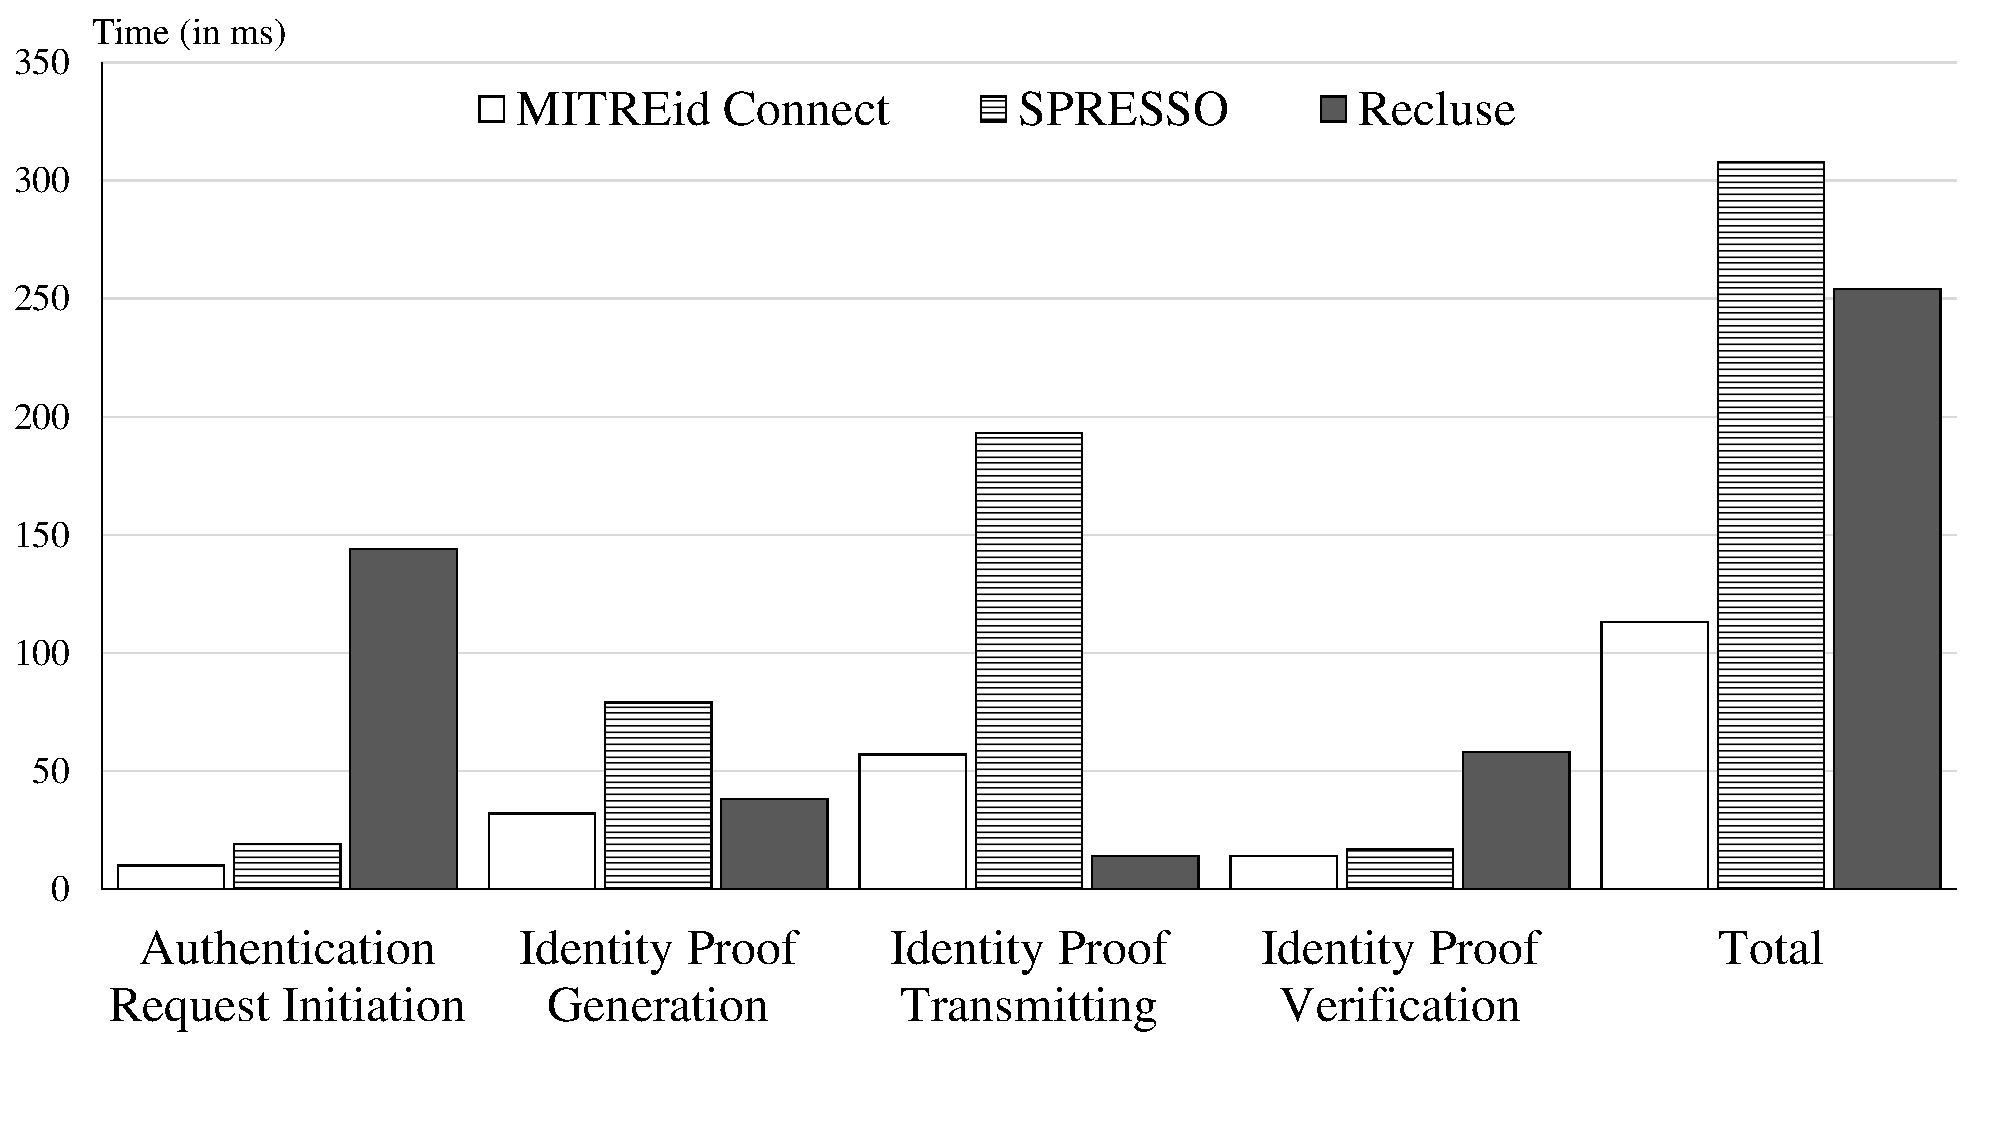
\includegraphics[width=0.9\linewidth]{fig/evaluation2.pdf}
  \vspace{-6mm}
  \caption{The Evaluation.}
  \label{fig:evaluation}
\vspace{-7mm}
\end{figure}

In the requesting, UPPRESSO requires 271 ms in total.
The significant overhead  in UPPRESSO occurs when opening the new window and downloading the script from IdP, which needs about 104 ms. This overhead could be reduced by implicitly conducting this procedure when the user visits the RP website.
SPRESSO needs 19 ms for the RP to obtain IdP's public key and encrypt its domain,
and MITREid Connect only needs 10 ms.



%估计能减少多少,
In the generation, UPPRESSO needs in total 34 ms, including computing $PID_U$, compared to MITREid Connect which only needs 32 ms.
SPRESSO requires 71 ms, as it implements the IdP based on node.js and therefore can only adopt a JavaScript cryptographic library, while others adopt a more efficient Java library.
%As the processings in SPRESSO and MITREid Connect are the same, the processing time in SPRESSO may be reduced to 32 ms.
%And, then the overall time in SPRESSO will be 269 ms, still larger than 254 ms in UPPRESSO.

%transmission & extraction
In the identity proof acceptance, UPPRESSO only needs  about 6 ms. % where the scripts relay the identity proof to the RP server, and RP server verifies and parses the proof.
MITREid Connect requires the IdP to send the identity proof to the RP's web page which then sends the proof to the RP server through a JavaScript function, and needs 71 ms.
SPRESSO needs the longest time (210 ms) due to the complicated processing at the user's browser.
  %which needs the browser to obtain identity proofs from the IdP, download the JavaScript program from a trusted entity (forwarder), execute the program to decrypt RP's endpoint, send identity proofs to this endpoint (an RP's web page) who finally transmits the proof to RP server.
%In the evaluation, the forwarder and IdP are deployed in one machine, which doesn't introduce performance degradation based on the observation. % as  FWD and IdP work sequently for one login.

%SPRESSO needs a trusted entity named FWD for transmitting the identity proof. We deployed FWD and IdP on the same machine to reduce transmitting delay between them, while the computation never becomes the bottleneck according to the observation.


%In the verification, UPPRESSO needs an extra calculation for $Account$, which then requires  58 ms,
% compared to 14 ms in MITREid Connect and 17 ms in SPRESSO.